\section{Introduction}
\label{sec:intro}

\begin{figure}[t]
	\centering
	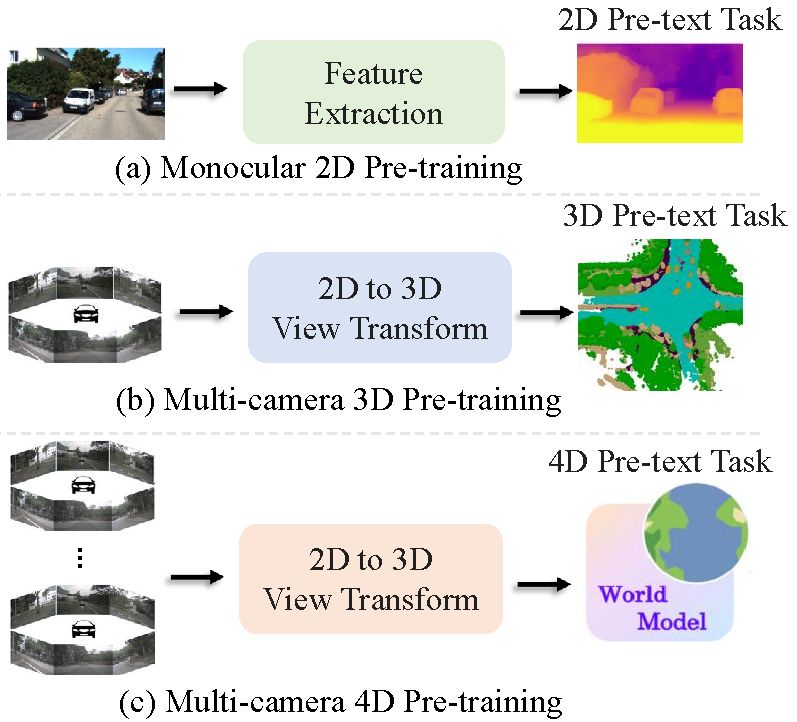
\includegraphics[width=0.4\textwidth]{figures/compare} 
	\caption{Comparison on different pre-training methods for vision-centric autonomous driving. (a) Monocular 2D pre-training with 2D pre-text tasks (\eg, 2D classification and depth estimation). (b) Multi-camera 3D pre-training via 3D scene reconstruction or 3D object detection. (c) The proposed 4D pre-training based on world models learns unified spatio-temporal representations.}
	%\vspace{-1em}
	\label{fig:compare1}
\end{figure}

Autonomous driving is a complex undertaking that relies on comprehensive 4D scene understanding~\cite{implicit,driveanywhere}. This demands the acquisition of a robust spatio-temporal representation that can address tasks involving perception, prediction, and planning~\cite{uniad}. Learning spatio-temporal representations is highly challenging due to the stochastic nature of natural scenes, the partial observability of the environment, and the diversity of downstream tasks~\cite{wu2023spatiotemporal,nunes2023temporal}. Pre-training plays a crucial role in acquiring a universal representation from massive data, enabling the construction of a foundational model enriched with common knowledge~\cite{bert,rebuffi2017learning,ponderv2,pimae,wang2023mvcontrast}.
However, research on pre-training for spatio-temporal representation learning in autonomous driving remains relatively limited.

Vision-centric autonomous driving has recently attracted increasing attention because of its lower cost~\cite{bevformer,bevdet,uniad,detr3d,petr,bevdepth,beverse}. However, as shown in Fig.~\ref{fig:compare1}, the existing vision-centric pre-training algorithms still predominantly rely on 2D pre-text tasks~\cite{resnet,dd3d} or 3D pre-text tasks~\cite{occnet,uniscene,unipad}. DD3D~\cite{dd3d} has demonstrated the effectiveness of depth estimation for pre-training. OccNet~\cite{occnet}, UniScene~\cite{uniscene}, and UniPAD~\cite{unipad} have further extended pre-training to 3D scene reconstruction. However, these algorithms overlook the importance of 4D representation for understanding self-driving scenes. 

We aim to employ world models to address 4D  representation for vision-centric autonomous driving pre-training. World models excel in representing an agent's spatio-temporal knowledge about its environment.~\cite{lecun,world_models}. In reinforcement learning, DreamerV1~\cite{dreamerv1}, DreamerV2~\cite{dreamerv2}, and DreamerV3~\cite{dreamerv3} employ world models to encapsulate an agent's experience within a predictive model, thereby facilitating the acquisition of a wide array of behaviours. MILE~\cite{mile} leverages 3D geometry as an inductive bias and learns a compact latent space directly from videos of expert demonstrations to construct world models in the CARLA simulator~\cite{carla}. ContextWM~\cite{contextwm} and SWIM~\cite{swim} pre-train world models with abundant in-the-wild videos to enhance the efficient learning of downstream visual tasks. More recently, GAIA-1~\cite{gaia} and DriveDreamer~\cite{drivedreamer} have constructed generative world models that harness video, text, and action inputs to create realistic driving scenarios using diffusion models. Unlike the aforementioned prior works on world models, our approach primarily focuses on harnessing world models to learn 4D representations for autonomous driving pre-training.

Driving inherently entails grappling with uncertainty~\cite{hu}. There are two types of uncertainty in ambiguous autonomous driving scenarios: aleatoric uncertainty, stemming from the stochastic nature of the world, and epistemic uncertainty, arising from imperfect knowledge or information~\cite{uncertainty}. How to leverage past experience to predict plausible future states, and estimate missing information about the state of the world for autonomous driving remains an open problem. In this work, we explore 4D pre-training via world models to deal with both aleatoric and epistemic uncertainties. Specifically, we design the Memory State-Space Model to reduce uncertainty within autonomous driving from two aspects. Firstly, to address aleatoric uncertainty, we propose the Dynamic Memory Bank module for learning temporal-aware latent dynamics to predict future states. Secondly, to mitigate epistemic uncertainty, we propose the Static Scene Propagation module for learning spatial-aware latent statics to provide comprehensive scene context. Furthermore, we introduce Task Prompt, which leverages semantic cues as prompts to tune the feature extraction network adaptively for different driving downstream tasks. 

To validate the performance of our proposed 4D pre-training approach, we conducted pre-training on the nuScenes~\cite{nuscenes} training set and the recently released large-scale 3D occupancy datasets, OpenScene~\cite{openscene}, followed by fine-tuning on the nuScenes training set. The experimental results demonstrate the superiority of our 4D pre-training approach when compared to 2D ImageNet pre-training~\cite{resnet}, 3D occupancy pre-training~\cite{occnet,uniscene}, and knowledge distillation algorithms~\cite{bevdistill}. Our 4D pre-training algorithm exhibited substantial improvements in vision-centric autonomous driving tasks, including 3D object detection, multi-object tracking, online mapping, motion forecasting, occupancy prediction, and planning. The main contributions of this work are listed below:
\begin{itemize}
	\item We present the first 4D pre-training method based on world models for real-world vision-centric autonomous driving, which learns a compact spatio-temporal representation from multi-camera driving videos.
	\item We design the Memory State-Space Model, which includes a Dynamic Memory Bank module for learning temporal-aware latent dynamics, a Static Scene Propagation module for learning spatial-aware latent statics, and a Task Prompt to condition feature extraction adaptively for various tasks.
	\item Extensive experiments indicate DriveWorld's pre-training aids in establishing new state-of-the-art performance in vision-centric perception, prediction, and planning tasks.
\end{itemize}

\begin{figure*}[t]
	\centering
	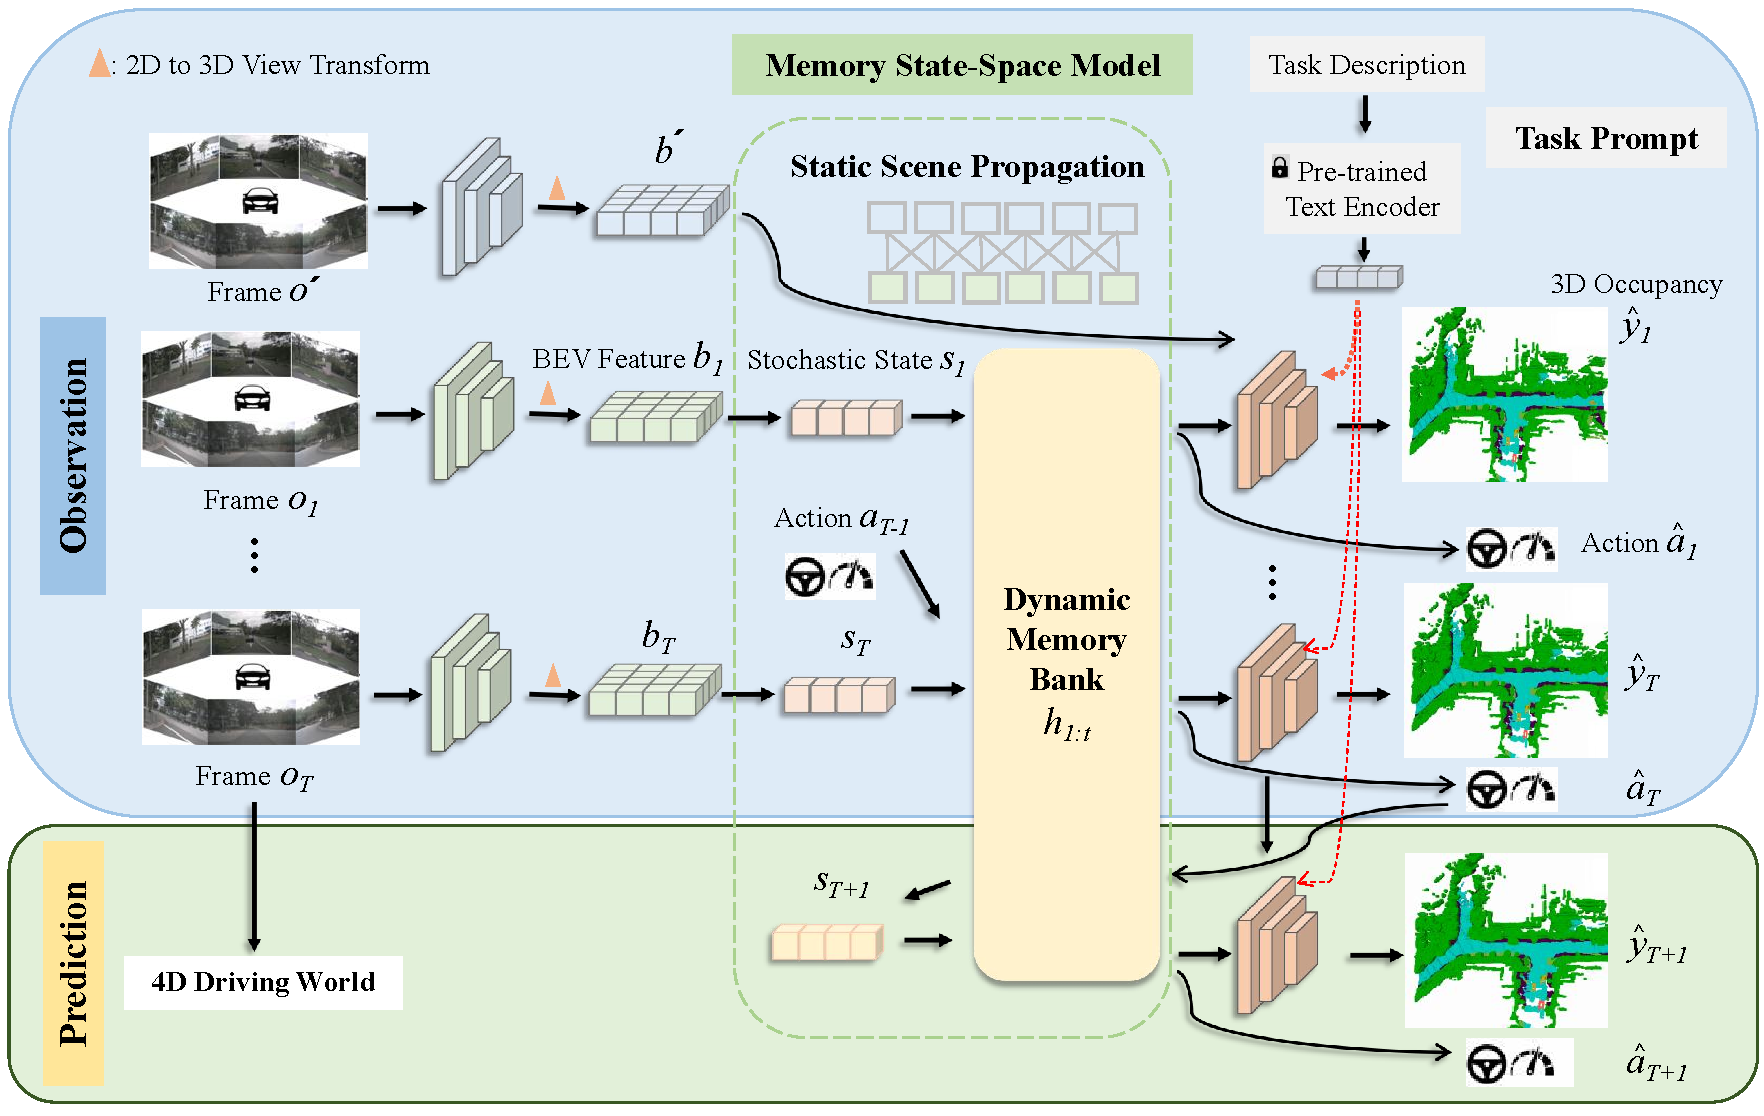
\includegraphics[width=0.86\textwidth]{figures/flowchart}
	\caption{\small{Overall framework of the proposed DriveWorld. Since autonomous driving heavily relies on the understanding of 4D scenes, our approach first involves the transformation of multi-camera images into a 4D space. Within the proposed Memory State-Space Model for spatio-temporal modelling, we have two essential components: the Dynamic Memory Bank, which learns temporal-aware latent dynamics for predicting future states, and the Static Scene Propagation, which learns spatial-aware latent statics to provide comprehensive scene context. This configuration facilitates the decoder's task of reconstructing 3D occupancy and actions for both the current and future time steps. Besides, we design the Task Prompt based on a pre-trained text encoder to adaptively decouple task-aware features for various tasks.}
	}
	%\vspace{-1em}
	\label{fig:flowchart}
\end{figure*}
